\section{Моделирование трения в контакте}

Вычислительная практика показала, что уравнения контакта в форме (\ref{3_4})
стабильно приводит к аварийному завершению процесса симуляции динамической 
модели ролика. Аналогичный результат получается, если в качестве уравнения 
контактирования использовать уравнение вида 
$$
v_n=0,
$$
где $v_n$ -- нормальная составляющая скорости точки контактирования, лежащей
на теле $B$, относительно тела $A$ (горизонтальной плоскости). И только 
уравнение вида
$$
\dot{v}_n=0
$$
приводит к требуемому результату -- корректной работе объекта контактирования
(реализованного в данном случае на языке Modelica~\cite{Fritzson}) в процессе 
симуляции модели. Заметим, что вся реализация процесса контактирования 
выполнена в предположении точечного <<твердого>> контакта твердых тел без 
какой-либо податливости.

Для каждого ролика модели омни-экипажа при контактировании <<включается>>
используемая здесь модель трения. Это <<простейший>> закон Амонтона -- Кулона
сухого трения. На самом деле вместо этого нами используется кусочно-линейная 
аппроксимация точного закона трения~\cite{Kosenko2006unilat}. Эта аппроксимация 
обеспечивает высокую точность вычисления движения тел на больших интервалах 
времени~\cite{Novozhilov1991}. Заметим, что и в общем случае реализация модели 
неудерживающей связи основывается на результатах, обозначенных в 
работе~\cite{Kosenko2006unilat}.

Конструкция омни-колеса такова, что в каждый данный 
момент времени имеется имеется только один контакт. Остальные ролики <<висят>>
над полом. При этом механическая связь между полом и, <<висящим>> на ободе
колеса, роликом не исчезает -- алгоритм отслеживания контакта продолжает 
работать, генерируя в качестве реакций нулевые усилия и моменты.

В случае фактического выполнения контакта помимо нормальной реакции вычисляется
также её касательная составляющая, симулирующая силу трения. Для касательного 
контактного усилия имеется (как и для нормального) множество различных моделей. 
Мы остановились на реализации простейшего случая -- модели сухого трения при 
одноточечном твердотельном контакте. При этом, как известно~\cite{Novozhilov1991}, 
идеальный <<сухой>> случай реализовать не удается. Вместо разрывной функции 
sign от касательной скорости относительного скольжения контактирующих 
поверхностей используется её регуляризованный в нуле вариант. В нашем случае 
вместо функции знака sign применяется функция линейного насыщения, имеющая в 
окрестности нуля <<крутой>> линейный участок. Для таких функций известен 
результат~\cite{Novozhilov1991} о близости аппроксимирующего движения и движения, соответствующего <<точному>> случаю разрывной функции sign.

В процессе отладки модели рассматривались автономные движения отдельного 
омни-колеса.

Заметим, что перед началом процесса редукции индекса системы 
дифференциально-алгебраических уравнений полной модели экипажа, реализованного
в программном обеспечении лаборатории динамического моделирования 
Dymola~\cite{Dymola}, эта модель составляется из: а) твердого тела платформы
омни--экипажа; б) трех твердых тел -- моделей омни--колес; в) двенадцати 
твердых тел роликов, размещенных на колесах. В соответствии, например, 
с~\cite{Kosenko2007} для каждого объекта, моделирующего твердое тело, 
реализуются шесть обыкновенных дифференциальных уравнений (ОДУ) Ньютона для
движения центра масс тела плюс семь ОДУ Эйлера для вращательного движения тела
вокруг центра масс. В последнем случае имеется четыре кинематических уравнения
Эйлера для кватерниона ориентации тела плюс три динамических уравнения Эйлера
для вектора угловой скорости твердого тела. В результате полная модель экипажа
задается системой ОДУ порядка $16\cdot 13=208$. Кроме этого, объекты 
механических связей могут генерировать дополнительные дифференциальные 
уравнения.

\begin{figure}[htb]
\centerline{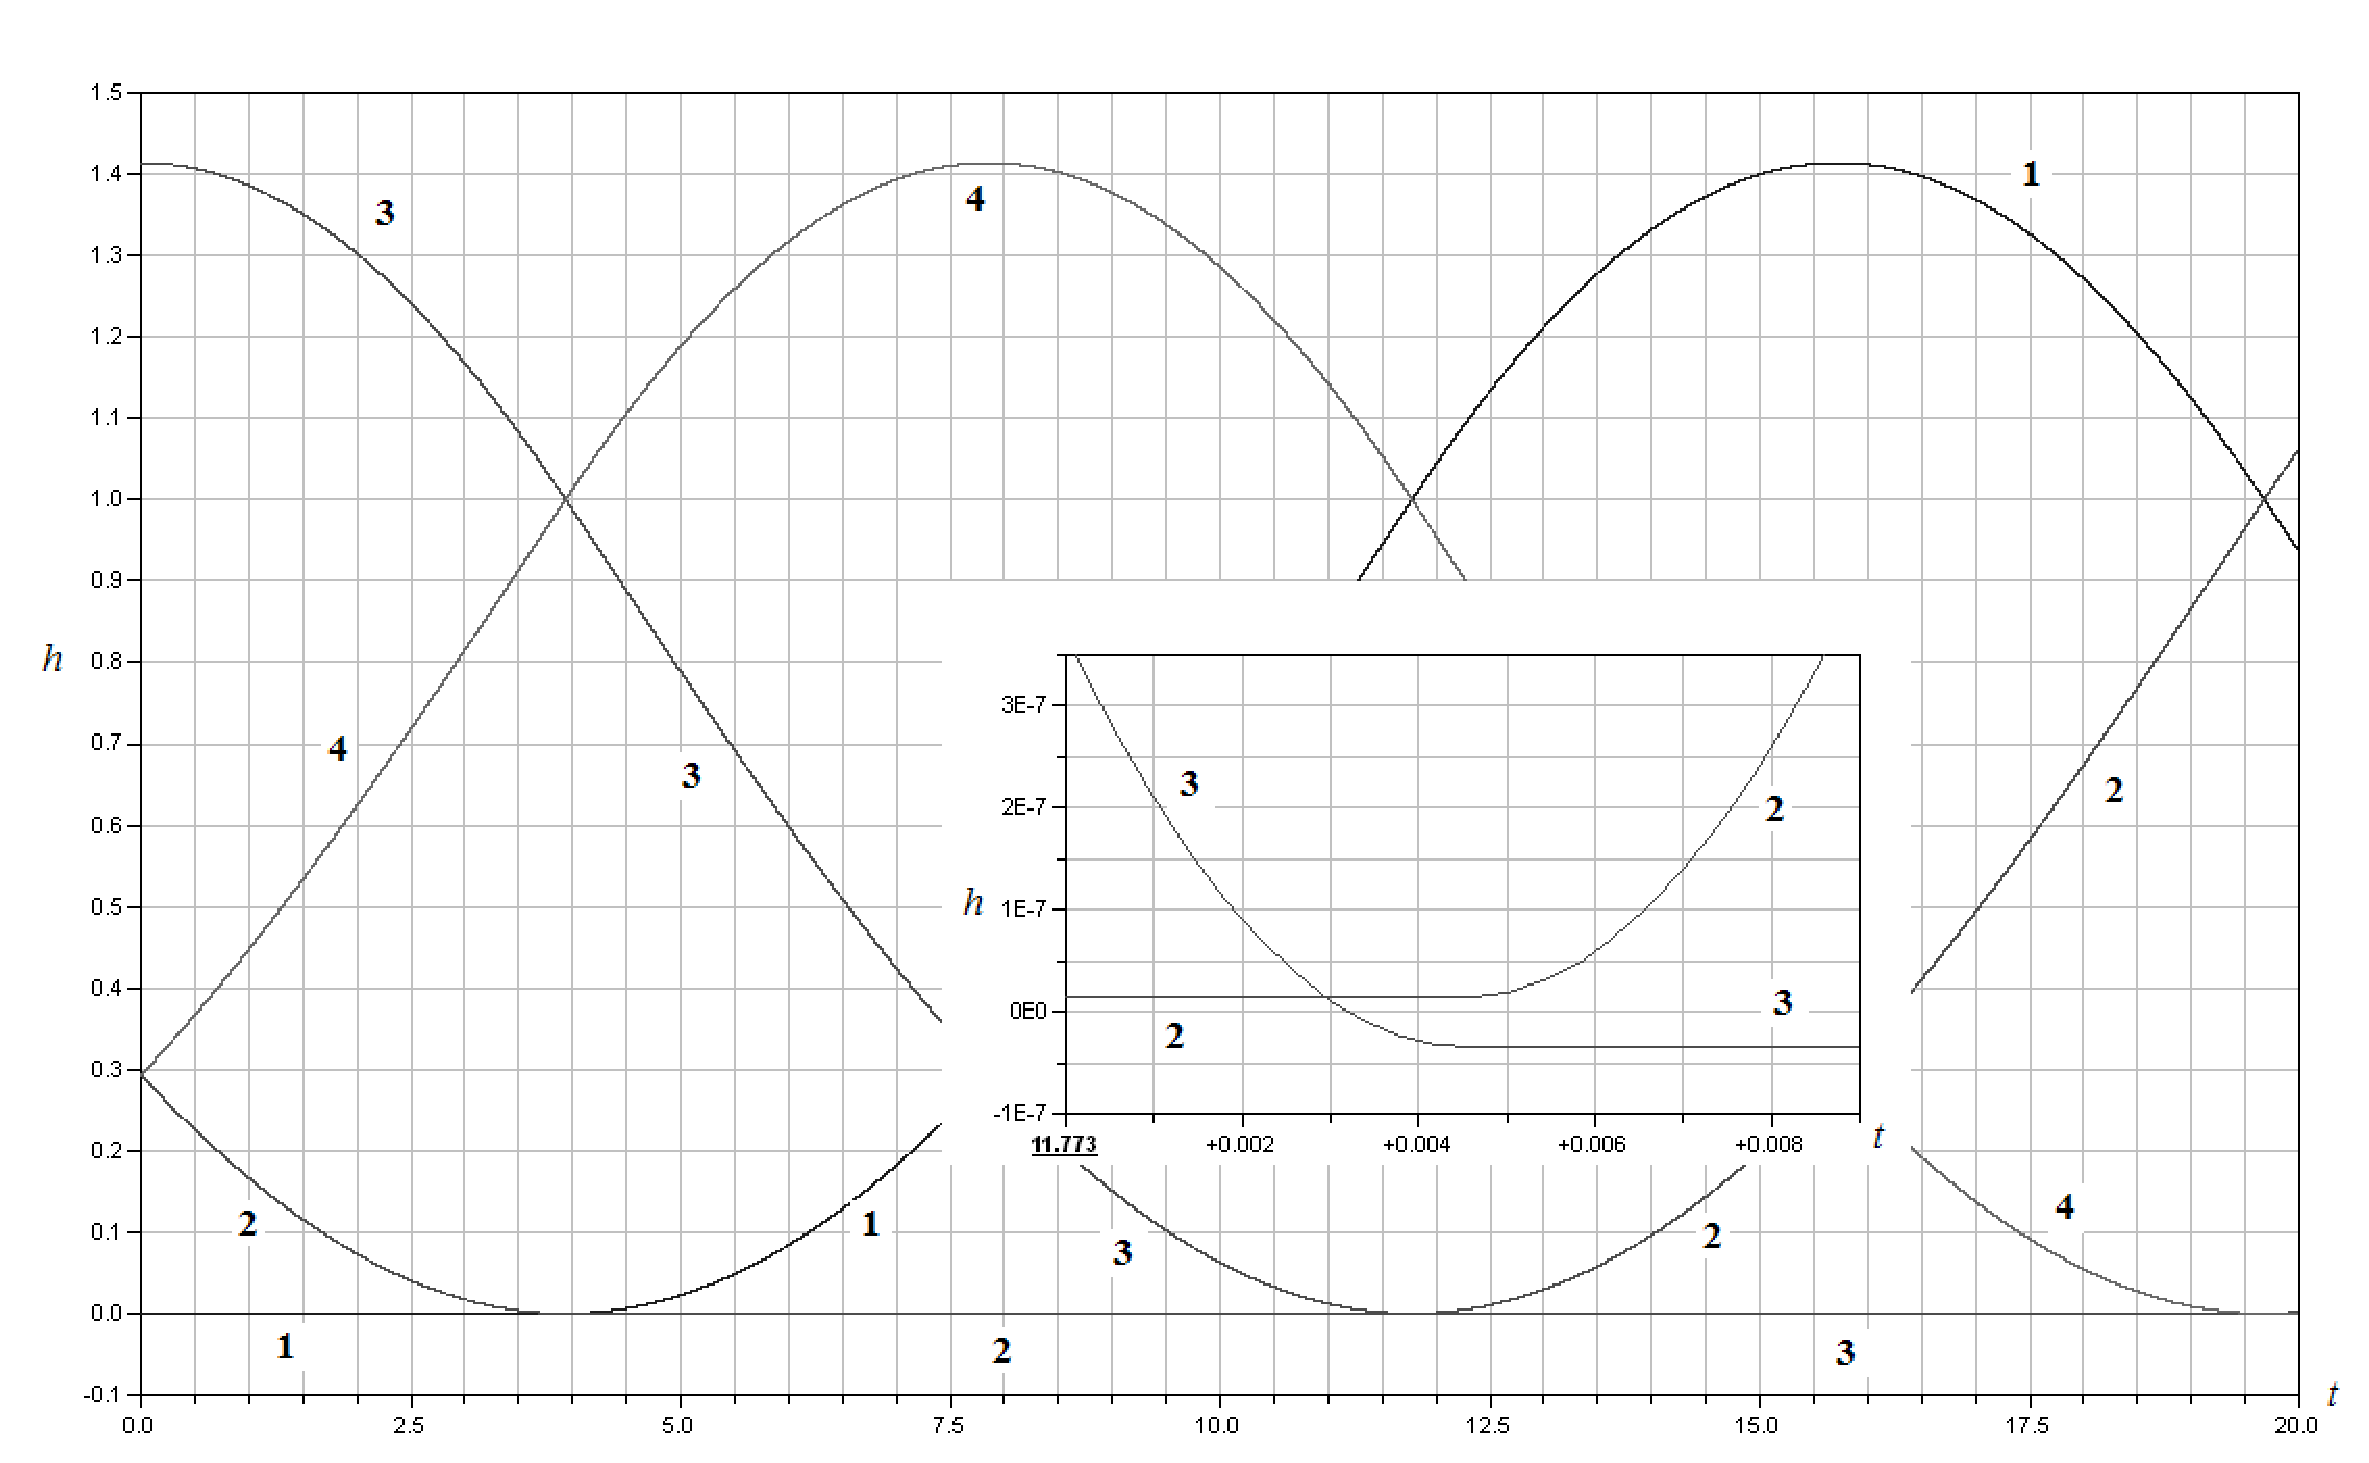
\includegraphics[width=15cm]{content/parts/3_friction/nd/Figure11.eps}}
\caption{Процесс замещения роликов в контакте.}
\label{fig1}
\end{figure}

Эволюция процесса контактирования для отдельного катящегося омни-колеса 
показана на Рис.~\ref{fig1}, где представлены зависимости функций расстояний 
$h$ (фактически -- высот) между горизонтальной плоскостью (полом) и роликами 
одного и того же колеса, находящимися в разных фазах (перед контактом, в 
контакте, после контакта). Функция высоты отдельного ролика помечена номером 
этого ролика. В увеличенном масштабе показан момент безударного гладкого 
переключения поверхностей контактирования роликов и горизонтальной плоскости.

Одновременно можно наблюдать точность соблюдения неудерживающей связи 
(Рис.~\ref{fig2}). Здесь обнаруживается процесс постепенного <<расползания>>
вычислительной ошибки -- расстояние между контактирующими телами медленно, для
каждого последующего ролика в контакте, увеличивается. В то же время, 
абсолютная величина ошибки остается пренебрежимо малой -- около $10^{-7}$
от единицы длины.

\begin{figure}[htb]
\centerline{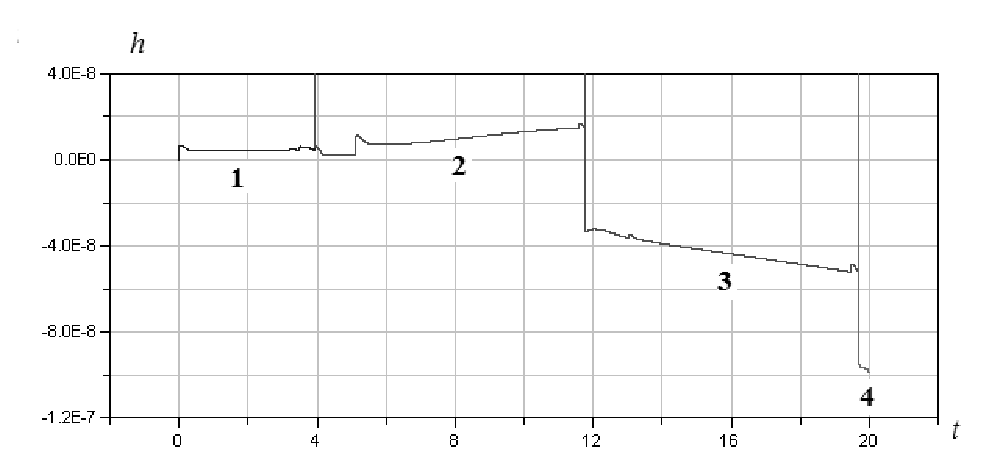
\includegraphics[width=15cm]{content/parts/3_friction/nd/Figure21.eps}}
\caption{Точность сохранения неудерживающей связи.}
\label{fig2}
\end{figure}
